\chapter{Iniciación}
\noindent En el presente capítulo se pretende describir el caso de estudio, los requerimientos funcionales, requerimientos no funcionales, perfiles de usuarios y la arquitectura base de la aplicación SaaS - Software as a Service.

\noindent El objetivo de esta fase en el Proceso Unificado Ágil, es obtener una máxima compresión cliente - equipo de desarrollo. Los requerimientos funcionales, el alcance del software a desarrollar (criterios de aceptación).

\section {Visión General - Caso de estudio}
\noindent Las empresas que ofrecen servicio de pedidos a domicilio a través de motorizados (mototaxis) en su mayor parte administran su negocio por medio de archivos Excel por lo cual tienen muchas limitaciones.
Para conocer el negocio y las respectivas actividades que realizan, se entrevistó a dos empresas de este rubro (Scooters, Ser). El flujo de trabajo desde que les llega el pedido consiste en:
\begin{itemize}
\item El encargo de recibir los pedidos, por cada pedido que llega, comunica a todos los motorizados por radio frecuencia.
\item Cada empresa tiene parqueos en los diferentes negocios de comidas en la mayoría y de acuerdo al orden de llegada tiene prioridad para que sean asignados a ese pedido.
\item En la mayor parte se tiene el siguiente caso para asignar un pedido. El pedido llega de algún restaurante o negocio de comidas o de cliente directo que quiere el pedido. Por decir, el restaurante de donde se debe recoger el pedido, la empresa de mototaxis no tiene parqueo por lo cual se debe ir preguntando quién quiere tomar el pedido, entonces los motorizados se reportan y dan su ubicación y si están disponibles y se ponen de acuerdo entre ellos quién podría tomar el pedido ya que se puede tener más de dos motorizados que quieran tomar ese pedido.
\end{itemize}
\indent Entre otras actividades administrativas dentro de las empresas de mototaxis:
\begin{itemize}
\item Cada motorizado debe pagar diariamente un monto por frecuencia recibida. en el transcurso del día deben reportarse en su central para iniciar su trabajo.
\item La empresa establece una multa diaria por inasistencia a todos los motorizados y se les recarga al momento que se reportan.
\item Al final del día (entre la 12:00 am), el encargado de la central realiza su informe de ingresos por frecuencia, cobro de multas y motorizados que no asistieron a trabajar.
\end{itemize}
\section{Identificación de requerimientos}
\noindent La identificación de requerimientos se basará en las actividades que realizan las empresas del rubro de servicios en mototaxis contemplando los siguientes escenarios principales para el desarrollo de la aplicación web (Software como un servicio - SaaS):
\begin{itemize}
\item \textbf{Administración de Pedidos}: Los operadores deben poder registrar los pedidos realizados por los clientes y asignar al motorizado que le corresponde.
\item \textbf {Administración de Mototaxis}: Los operadores deberán poder registrar, actualizar información o deshabilitar a los respectivos motorizados de la empresa. También podrán registrar el pago por frecuencia diaria o las multas por inasistencia.  
\item \textbf{Administración de usuarios}: Cada Empresa de mototaxis solo podrá tener una cuenta administrador y  varias cuentas de operadores.
\item \textbf{Administración de Seguridad}: El acceso a la información y las diferentes operaciones que puedan realizar los usuarios deberán ser controlados bajo perfiles de usuarios (administrador de la empresa y operadores).
\end{itemize}

\section{Requerimientos funcionales}

\noindent Los requerimientos funcionales fueron agrupados de acuerdo a las áreas de administración detectadas en común en las empresas y también se consideró la definición de la administración de seguridad que tiene que ver más con la aplicación web.

\begin{table}[H]
	\centering
    \begin{tabular}{ |c|p{10cm}|c| }
	  \hline
	  \rowcolor{indigo-dark} \multicolumn{3}{|c|}{ \textcolor{white}{\textbf{Administración de Pedidos}}} \\
	  \hline
	  \rowcolor{indigo-light} \textbf{N\#} & \centering \textbf{Descripción} & \textbf{Prioridad} \\
	  \hline
	  1 & El usuario con perfil de operador podrá registrar los pedidos realizados por los clientes. & Alta\\
	  \hline
	  2 & El usuario con perfil de operador tendrá la opción de poder consultar a qué mototaxi corresponde la asignación del pedido. & Media \\
	  \hline
	  3 & El usuario con perfil de operador podrá ver la lista de pedidos realizados en el dia.   & Baja \\
	  \hline
	\end{tabular}
	\caption{Requerimientos de la administración de pedidos}
\end{table}

\begin{table}[H]
	\centering
    \begin{tabular}{ |c|p{10cm}|c| }
	  \hline
	  \rowcolor{indigo-dark} \multicolumn{3}{|c|}{ \textcolor{white}{\textbf{Administración de Mototaxis}}} \\
	  \hline
	  \rowcolor{indigo-light} \textbf{N\#} & \centering \textbf{Descripción} & \textbf{Prioridad} \\
	  \hline
	  4 & El usuario con perfil de operador podrá registrar nuevos motorizados a la respectiva empresa a la cual corresponde. & Alta \\
	  \hline
	  5 & El usuario con perfil de operador podrá registrar el cobro por frecuencia diaria realizada a los respectivos mototaxis. & Alta \\
	  \hline
	  6 & El usuario con perfil de operador podrá registrar el cobro por multa de inasistencia a los respectivos motorizados de la empresa. & Alta \\
	  \hline
	  7 & El usuario con perfil de operador podrá listar los mototaxis correspondientes a la empresa & Baja \\
	  \hline
	\end{tabular}
	\caption{Requerimientos de la Administración de Mototaxis de las respectivas empresas}
\end{table}

\begin{table}[H]
	\centering
    \begin{tabular}{ |c|p{10cm}|c| }
	  \hline
	  \rowcolor{indigo-dark} \multicolumn{3}{|c|}{ \textcolor{white}{\textbf{Administración de Usuarios}}} \\
	  \hline
	  \rowcolor{indigo-light} \textbf{N\#} & \centering \textbf{Descripción} & \textbf{Prioridad} \\
	  \hline
	  8 & El usuario con perfil de administrador es el único que puede crear cuentas de operadores para la empresa correspondiente. & Alta\\
	  \hline
	  9 & El usuario con perfil de administrador solo podrá ver la información relacionada a los operadores de la empresa, ingresos diarios y mensuales por cobro por frecuencia y multas por inasistencia de los mototaxis. & Media \\
	  \hline
	  10 & La aplicación web deberá proporcionar la opción que los usuarios puedan  cambiar sus datos personales. & Baja \\
	  \hline
	\end{tabular}
	\caption{Requerimientos de los perfiles de usuarios para las empresas}
\end{table}

\begin{table}[H]
	\centering
    \begin{tabular}{ |c|p{10cm}|c| }
	  \hline
	  \rowcolor{indigo-dark} \multicolumn{3}{|c|}{ \textcolor{white}{\textbf{Administración de Seguridad}}} \\
	  \hline
	  \rowcolor{indigo-light} \textbf{N\#} & \centering \textbf{Descripción} & \textbf{Prioridad} \\
	  \hline
	  11 & La aplicación web deberá controlar el acceso a la información a través de la autentificación de usuarios y mostrará el menú de operaciones que puede realizar el usuario de acuerdo al perfil de usuario (Administrador u Operador). & Alta\\
	  \hline
	  12 & La aplicación web deberá controlar las operaciones de acuerdo al tipo de perfil  de usuario que define por cada operación en los recursos de información con los accesos de (lectura, escritura, eliminación y/o actualización). & Alta\\
	  \hline
	  13 & La aplicación web deberá controlar el acceso a la información a los diferentes usuarios que solo puedan ingresar a la información de la empresa a la cual pertenecen. & Alta \\
	  \hline
	  14 & La aplicación web deberá permitir crear una cuenta empresa en conjunto con la cuenta administrador. & Media \\
	  \hline
	  15 & La aplicación web deberá proporcionar las opciones de iniciar sesión y cerrar session. &  Media\\
	  \hline
	  16 & La aplicación web deberá permitir a los usuarios cambiar contraseña. &  Baja \\
	  \hline
	\end{tabular}
	\caption{Requerimientos de Seguridad de la aplicación web}
\end{table}

\section{Perfiles de usuarios}
\noindent La aplicación web define dos tipos de perfiles de usuarios (Administrador y Operador). Cada perfil de  usuario puede realizar cierto número de operaciones dentro la aplicación web.
\noindent los perfiles de usuarios definidos son:
\begin{itemize}
\item \textbf{Administrador}: El perfil de administrador es creado al mismo tiempo cuando se crea la cuenta de la empresa en la aplicación web. Este perfil de usuario está enfocado a administrar las cuentas de los operadores correspondientes a la empresa, reportes de ingresos por cobro de frecuencia y multas y ver los respectivos mototaxis registrados.
\begin{figure}[ht]
  \centering
  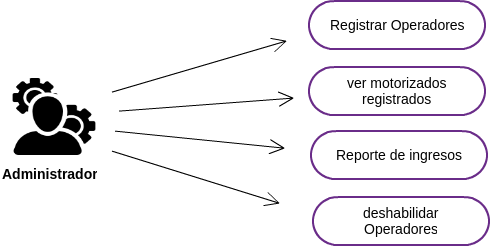
\includegraphics[width=8cm, height=4cm]{chapter3-admin-profile.png}
  \caption{Acciones que puede realizar un Administrador [Elaboracion propia ]}  
\end{figure}
\item \textbf{Operador}: El perfil de Operador está enfocado a registrar nuevos motorizados, registrar pago de frecuencias y multas. Este perfil de usuario está enfocado a al registro de las diferentes transacciones o actividades diarias que se realizan en la empresa.
\begin{figure}[ht]
  \centering
  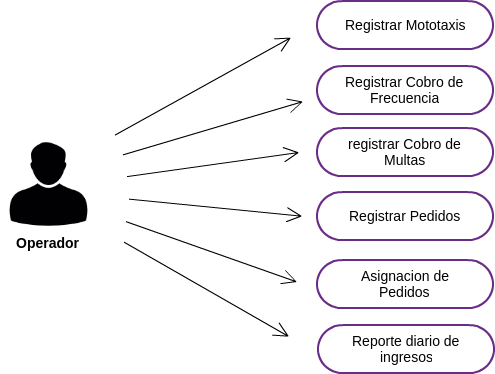
\includegraphics[width=8cm, height=7cm]{chapter3-operator-profile.png}
  \caption{Acciones que puede realizar un Operador [Elaboracion propia ]}  
\end{figure}
\end{itemize}

\section{Requerimientos no funcionales}
\noindent Según la definición de [Swebok, 2014], Los requerimientos no funcionales algunas veces son conocidos como las restricciones del proyecto o requerimientos de calidad. Los requerimientos no funcionales pueden ser clasificados en requerimientos de rendimiento, mantenimiento, seguridad, fiabilidad, interoperabilidad y muchos otros.

\noindent Los requerimientos no funcionales que se considera en el proyecto estan agrupados de la siguiente manera: atributos del Software, consideraciones para los entornos de ejecución y la tecnología a utilizar.

\subsection{Atributos de Software}
\noindent Según [Sommerville, 2005], los productos de software tienen un cierto número de atributos que reflejan la calidad del software. Estos atributos reflejan su comportamiento durante su ejecución y la estructura organizacional del código fuente y la documentación asociada.
\noindent El software a desarrollar deberá enfocarse en los siguientes atributos:
\begin{itemize}
\item \textbf{Rendimiento}: El rendimiento del software por cada acción o petición que realiza un usuario dentro del sistema debe cumplir el siguiente criterio: el tiempo de respuesta deberá ser menor a 5 segundos.
\item \textbf{Concurrencia}: El software debe estar diseñado para soportar múltiples usuarios que estén usando el software al mismo tiempo.
\item \textbf{Escalabilidad}: El software debe ser escalable de acuerdo al siguiente criterio. El número de usuarios incrementa 100 a 1000 usuarios, entonces se puede incrementar los recursos de hardware y el rendimiento del software deberá ser casi similar soportando 1000 usuarios a soportar 100 usuarios con menos recursos de hardware. 
\item \textbf{Mantenimiento}: El software debe ser mantenible considerando los siguientes criterios: comprensión fácil de la estructura del código (diseño arquitectónico), debidamente documentado en código fuente donde se requiera y documentos técnicos adicionales si fuera necesarios y automatización de tareas repetitivas en el proceso de desarrollo.  
\end{itemize}

\subsection{Tecnología}
\noindent La tecnología a utilizar para el desarrollo del proyecto es la siguiente:

\begin{table}[H]
	\centering
    \begin{tabular}{ |P{4cm}|p{10cm}| }
	  \hline
	  \rowcolor{indigo-dark} \multicolumn{2}{|c|}{ \textcolor{white}{\textbf{Tecnología}}} \\
	  \hline
	  \rowcolor{indigo-light} \textbf{Nombre} & \centering \textbf{Descripción}
	  \tabularnewline \hline
	  Entornos de Ejecución en Heroku & Heroku es una plataforma en la nube basado en un sistema de contenedores, con servicios de datos integrados y un potente ecosistema, para implementar y ejecutar aplicaciones modernas.
	  \tabularnewline \hline
	  Repositorio de código fuente en Github & Github es una plataforma de desarrollo colaborativo para alojar proyectos utilizando el sistema de control de versiones Git. 
	  \tabularnewline \hline
	  Plataforma de desarrollo en Nodejs & Nodejs es una plataforma de desarrollo que utiliza como lenguaje de programación Javascript y define un modelo asíncrono manejado por eventos lo cual nos permite crear aplicaciones escalables. 
	  \tabularnewline \hline
	  Base de datos en MongoDB & MongoDB es un manejador de base de datos NoSQL orientado a documentos. 
	  \tabularnewline \hline
	Integración Continua con Travis CI & Travis Ci es un servicio en la nube para realizar integración continua. Se puede sincronizar con los repositorios en Github  y ejecutarse apenas se modifique algo en el repositorio, también se integra a Heroku para hacer los desplazamientos de nuevos cambios en el código a los entornos de ejecución. 
	  \tabularnewline \hline
	\end{tabular}
	\caption{Tecnología a utilizar en el desarrollo del proyecto}
\end{table}

\section{Arquitectura del Software}
\noindent El sistema estará compuesto por dos subsistemas, la aplicación web y el servicio web. Para el almacenamiento de datos se aplicará una arquitectura de datos multi tenant. El servicio web es el medio para acceder a los datos y realizar operaciones. La aplicación web consume los recursos que le proporciona el servicio web.

\noindent A continuación se tiene una descripción gráfica de la Arquitectura a implementar. 
\begin{figure}[H]
  \centering
  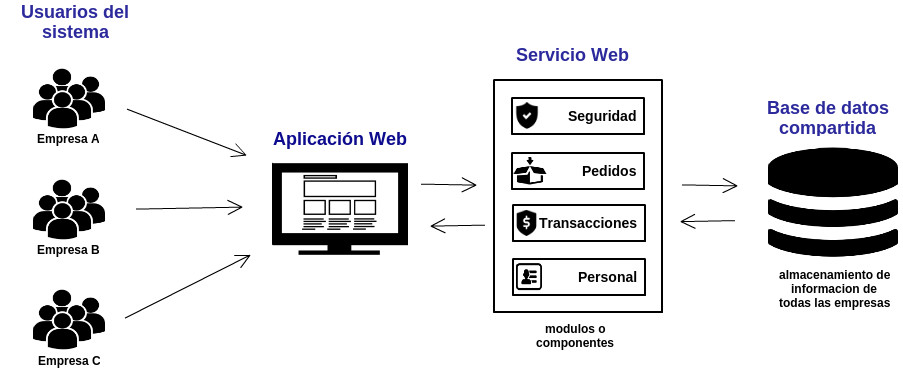
\includegraphics[width=15cm, height=5cm]{chapter3-architecture-of-the-project.png}
  \caption{Arquitectura aplicación SaaS - empresas de pedidos [Elaboración propia]}  
\end{figure}
   
\subsection{Aplicación Web}
\noindent La aplicación web es un cliente que consume recursos que le proporciona el servicio web. La forma como va a mostrar la información estará limitado por los recursos que le proporciona el servicio web.

\noindent A continuación se presenta la arquitectura que tendrá la aplicación web.
\begin{figure}[H]
  \centering
  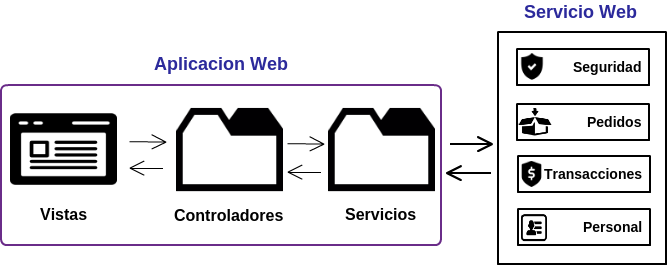
\includegraphics[width=12cm, height=4cm]{chapter3-architecture-web-app.png}
  \caption{Arquitectura de la aplicación web [Elaboración propia]}  
\end{figure} 

\noindent Los \textbf{Controladores} se encargan de proveer información a las vistas para lo cual hacen uso de los \textbf{Servicios} que su finalidad es conectarse con el servicio web y consumir los recursos que están disponibles.

\subsection{Servicio Web}
\noindent Para la implementación de los servicios web se realizará bajo la tecnología REST, según [Richardson \& Ruby, 2007] REST - REpresentational State Transfer, es un tipo de arquitectura que se apoya en el estándar HTTP. REST nos permite crear servicios compatibles con cualquier dispositivo o cliente HTTP.

\noindent En un servicio REST, se define los recursos accesibles por identificadores y en los cuales se realizará las operaciones como ser (Agregar, Actualizar, Eliminar u Obtener)

\noindent La arquitectura para los servicios web estará conformada por capas, donde cada capa sólo conoce lo que hace la capa inmediatamente inferior. Cada capa encapsula su implementación y ofrece una interfaz para que la capa superior pueda comunicarse.
\begin{figure}[H]
  \centering
  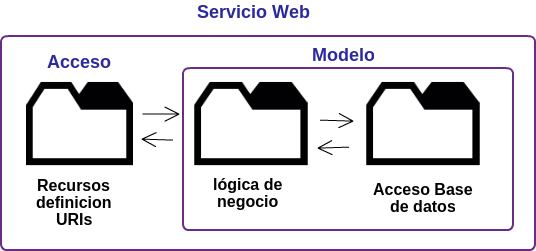
\includegraphics[width=12cm, height=4cm]{chapter3-architecture-web-service.png}
  \caption{Arquitectura del servicio web [Elaboración propia]}  
\end{figure}
 \noindent En la \textbf{capa de acceso} se define todos los recursos que proporcionará el servicio web. Un URI - Uniform Resource Identifier, nos permiten identificar de forma única un recurso.

\noindent En la \textbf{capa de modelo} se definirá la las reglas de negocio y los esquemas de la base de datos. 

\subsection{Arquitectura de Datos Multi-Tenant}
\noindent Una prioridad alta para una aplicación SaaS, es definir la arquitectura de datos para almacenar la información de los diferentes clientes que usen la aplicación. el almacenamiento de datos debe ser robusta y segura lo suficiente para que los clientes puedan ceder el control de los datos empresariales a la aplicación SaaS.

\noindent En el siguiente articulo [Multi Tenant, msdn 2006] habla sobre tres estrategias para implementar una arquitectura de Datos, tomando dos extremos: Isolar datos y compartir datos.

\noindent Las estrategias para implementar una arquitectura de datos son las siguientes:
\begin{itemize}
\item Una base de datos para cada cliente 
\item Una base de datos única pero con diferentes esquemas para cada cliente
\item Una única base de datos para todos los clientes
\end{itemize}

\noindent Para el desarrollo de la aplicación SaaS se utilizara la estrategia textbf{una base de datos para todos los clientes} con las siguientes restricciones:
\begin{itemize}
\item Para almacenar la información se deberá diferenciar con un código único para cada cliente empresa.
\item La seguridad al acceso de información debe ser controlada, de tal forma que una empresa solo pueda ingresar a la información relacionada a esa empresa.
\end{itemize}

\noindent La ventajas de tener una base de datos para todos los clientes son los siguientes:
\begin{itemize}
\item Minimizar el costo inicial en cuanto a recursos de hardware. una base de datos se crea con un mínimo de memoria en disco duro y en los planes de plataformas en la nube hay un costo por capacidad de almacenamiento.
\item Minimizar el costo de mantenimiento o administración las bases de datos en cuanto a sacar respaldo de datos y restauración. Como se tiene solo una base de datos se reduce este costo y la complejidad de mantenimiento.  
\end{itemize} 


